\documentclass[11pt, oneside]{article}   	% use "amsart" instead of "article" for AMSLaTeX format
\usepackage[margin=1in]{geometry}                		% See geometry.pdf to learn the layout options. There are lots.
\geometry{letterpaper}                   		% ... or a4paper or a5paper or ... 
%\geometry{landscape}                		% Activate for rotated page geometry
%\usepackage[parfill]{parskip}    		% Activate to begin paragraphs with an empty line rather than an indent
\usepackage{graphicx}				% Use pdf, png, jpg, or eps§ with pdflatex; use eps in DVI mode
								% TeX will automatically convert eps --> pdf in pdflatex		
\usepackage{amssymb}
\usepackage{awesomebox}
%SetFonts

%SetFonts

\usepackage{amsmath}
%\DeclareMathOperator{\mod}{mod}
\let\emptyset\varnothing

\newcommand{\reals}{\mathbb{R}}
\newcommand{\realsText}{$\mathbb{R}$}
\newcommand{\ints}{\mathbb{Z}}
\newcommand{\intsText}{$\mathbb{Z}$}

\title{Homework 2}
\author{Discrete Structures 2}
\date{due: 21 February 2023, 8:00am}							% Activate to display a given date or no date

\begin{document}
\maketitle
%\section{}
%\subsection{}

Your task for this homework will be to answer the following questions without using any calculating resources. 
Your responses should be submitted via blackboard by the due date above as a PDF (submissions in any other format will be returned to the user and a resubmissions will be requested). 
You are free to use whatever tools you would like to generate the response document: 
scanned hand-written paper, 
tablet generated hand-written, 
microsoft word (with this option, please use the equation editor to correctly format your responses), 
\LaTeX, etc.
Your TA, IA, and Instructor are available to help during their designated office hours or via email 
(note that emails sent during non-business hours may not be responded to until the next working day). 

\importantbox{
\textbf{Note:} all of these questions are on topics from chapters 3 and 4; thus you will not be proving by induction in this homework assignment. 
}
\begin{enumerate}
% 3.148-151
\item Let $F$ denote the set of all functions $f : \reals \rightarrow \reals$ taking real numbers as input and producing real numbers as output. 
(For one example, $plusOne(x) = x + 1$ is a function $plusOne : \reals \rightarrow \reals$, so $plusOne\in F$.) 
Determine the truth of the following propositions, and justify your answer. 
\begin{enumerate}
\item $\forall c \in \reals \left[\exists f \in F : f(0) = c\right]$
\item $\exists f \in F \left[\forall c \in \reals : f(0) = c\right]$
\item $\forall c \in \reals \left[\exists f \in F : f(c) = 0 \right]$
\item $\exists f \in F \left[\forall c \in \reals : f(c) = 0 \right]$
\end{enumerate}

%3.160-163
\item 
Let $P \in \left\{0,1\right\}^{n\times m}$ be a 2-dimensional array of the pixels of a black-and-white image: 
for every $x$ and $y$, the value of $P[x, y] = 0$
if the $\langle x, y\rangle$-th pixel is black, and $P[x, y] = 1$ if it’s white. 
Translate these statements into predicate logic:
\begin{enumerate}
\item Every pixel in the image is black
\item There is at least one white pixel
\item Every row has at least one white pixel
\item There are never two consecutive white pixels in the same column
\end{enumerate}

%4.36
\item Prove that the binary representation of any odd integer ends with a 1.
\tipbox{hint: you will need to rely on how we represent a number in binary and modulus}

%4.53
\item Prove the following by \textbf{contrapositive}: For $n\in\ints^{\ge0}$. If $2n^4 +n+5$ is odd, then $n$ is even.

%4.57
\item Prove the following by \textbf{contradiction}: Suppose $12x+3y=254$, for real numbers $x$ and $y$. Then either $x$ or $y$ (or both) is not an integer.

%4.62
\item \textit{Disprove} the following by \textbf{counterexample}: If $x−y$ is rational, then $x$ and $y$ are rational.

%%4.95
%\item For the following false claim and a bogus proof of that false claim 
%(a) identify the precise error in the proof, and 
%(b) give a counterexample to the claim. 
%(Note that saying why the claim is false does not address (a) in the slightest—it would be possible to give a bogus proof of a true claim!)
%
%\textbf{False Claim 1.} 
%Let $n$ be a positive integer and let $p, q \in \ints^{\ge2}$ , where $p$ and $q$ are prime. 
%If $n$ is evenly divisible by
%both $p$ and $q$, then $n$ is also evenly divisible by $pq$.
%
%\textbf{Bogus proof.} 
%Because $p | n$, there exists a positive integer $k$ such that $n = pk$. 
%Thus, by assumption, we know that $q | pk$. 
%Because $p$ and $q$ are both prime, 
%we know that $p$ does not evenly divide $q$, and thus the only way that $q | pk$ can hold is if $q | k$. 
%Hence $k = q\ell$ for some positive integer $\ell$, and thus $n = pk = pq\ell$. 
%Therefore $pq | n$.

%4.108
\item 
\label{q:triangles}  Here is a (nonobviously) bogus proof of the (obviously) bogus claim that $0=1$.
Identify precisely the flaw in the argument. 

\textbf{Proof that 0 = 1.} 
Consider the four shapes in Figure~\ref{fig:triangles}a, 
and the two arrangements thereof in  Figure~\ref{fig:triangles}b. 
The area of the triangle in the first configuration is $\frac{13\cdot5}{2} = \frac{65}{2}$, 
as it forms a right triangle with height 5 and base 13. 
But the second configuration also forms a right triangle with height 5 and base 13 as well, and therefore it too has area $\frac{65}{2}$. 
But the second configuration has one unfilled square in the triangle, and thus we have
\[
\begin{aligned}
0 =& \frac{65}{2} - \frac{65}{2}\\
=& \text{area of the second bounding triangle} - \text{area of the first bounding triangle}\\
 =& (1 + \text{area of four constituent shapes}) - (\text{area of four constituent shapes})\\
 =& 1.
 \end{aligned}
 \]

\tipbox{hint: you may want to look at where exactly the 3 objects meet along the ``hypotenuse''}
 
 \begin{figure}[h!]
\begin{center}
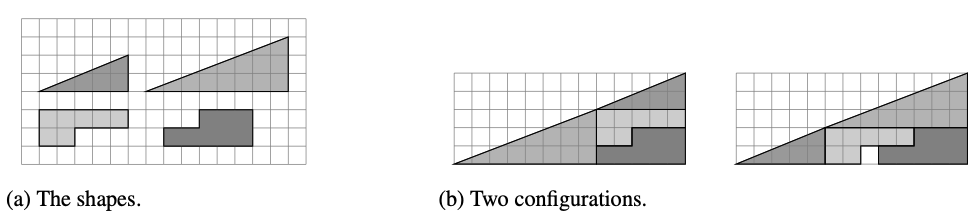
\includegraphics[width=\columnwidth]{DS2-HW2-triangles}
\caption{Figures for Question~\ref{q:triangles}}
\label{fig:triangles}
\end{center}
\end{figure}


\end{enumerate}

\end{document}